\chapter{Introduzione}
\chaptermark{Introduzione}
\label{chap:introduction}

Il cloud computing è un modello di erogazione di servizi che consente di gestire l'infrastruttura informatica necessaria per rendere disponibili applicazioni, dati e servizi online in modo rapido, efficiente e flessibile. Grazie al cloud computing, le risorse informatiche come server, storage e software possono essere facilmente scalate per rispondere alle esigenze delle organizzazioni e degli utenti finali, consentendo un accesso sicuro e veloce ai servizi e alle applicazioni da qualsiasi dispositivo connesso a Internet. La rapidità e velocità con cui il cloud computing eroga questi servizi è data dalle tecnologie che lo compongono.
\\
In questo contesto andremo a discutere di una emergente tecnologia, chiamata \textbf{WASI (WebAssembly System Interface)}\footnote{\url{https://wasi.dev/}} e come questa possa essere considerata la terza ondata del cloud computing\cite{cloudcomputing-thirdwave}.
Grazie a WASI, è possibile eseguire applicazioni in un ambiente isolato e sicuro, senza la necessità di dover conoscere il sistema operativo sottostante. È stato progettato per essere altamente portabile, consentendo alle applicazioni di essere eseguite in modo efficiente su qualsiasi piattaforma.
\\
Nasce e si sviluppa sopra ad una tecnologia già esistente: \textbf{WebAssembly} (o \textbf{Wasm}). Quest'ultima è un'innovativa tecnologia nata con l'obiettivo di migliorare le prestazioni delle applicazioni web \textbf{sul browser}. È stata progettata con l'intento di superare le limitazioni poste da Javascript. In particolare, si propone di essere veloce, efficiente e portabile, oltre che retro-compatibile con le tecnologie già esistenti. Va notato che WebAssembly non è pensato per sostituire JavaScript, ma piuttosto per migliorare le aree in cui quest'ultimo presenta alcune lacune: come il rendering 3D, il video editing, giochi in-browser e così via.
\\\\
WASI eredita tutte queste caratteristiche da Wasm e le utilizza per lo sviluppo di applicazioni \textbf{al di fuori} dei browser.
\\\\
Di seguito andremo ad approfondire WASI ed esporremo come rappresenti una tecnologia estremamente promettente per il futuro nell’ambito del cloud computing in particolare, sebbene sia ancora in fase di sviluppo e di adozione.

\clearpage

\section{Un focus su WebAssembly}
\label{sec:webassembly}
Tradizionalmente, l'unico linguaggio utilizzabile all'interno dei browser era JavaScript, perfetto per la creazione di interfacce utente ma non per operazioni che richiedono una complessità maggiore. WebAssembly è stato progettato per essere un formato di esecuzione più efficiente, veloce e sicuro rispetto a JavaScript, da usare in combinazione con esso\cite{webassembly-concepts}.
\\
In sintesi, WebAssembly è un formato binario (.wasm) progettato per essere eseguito da una macchina virtuale integrata all'interno dei browser. Grazie alla sua natura binaria, è possibile utilizzare diversi linguaggi di programmazione, come C, C++ e Rust, che supportano questo formato.
\\
Ogni file .wasm contiene un \textbf{modulo}, che può essere visto come un'unità di codice autonomo, composto da funzioni, dati e altre risorse. Il modulo viene eseguito all'interno della macchina virtuale del browser in modalità sandboxed, che garantisce l'isolamento e la sicurezza dell'esecuzione.
\\
Ogni rappresentazione binaria possiede anche una duale rappresentazione testuale chiamata \textbf{WebAssembly Text Format (.wat)}. Questo formato ha una sintassi simile ai linguaggi Assembly, il che lo rende più leggibile per gli esseri umani rispetto al formato binario. Un file .wat è costituito da una serie di istruzioni che definiscono la struttura del modulo organizzate in sezioni.
\\
Il vantaggio di avere una rappresentazione testuale come il formato .wat è che può aiutare gli sviluppatori a comprendere meglio la struttura e il funzionamento dei moduli, anche se non sono esperti nel linguaggio Assembly o nell'architettura della CPU.

\begin{figure}[h]
    \centering
    \captionsetup{justification=centering}
    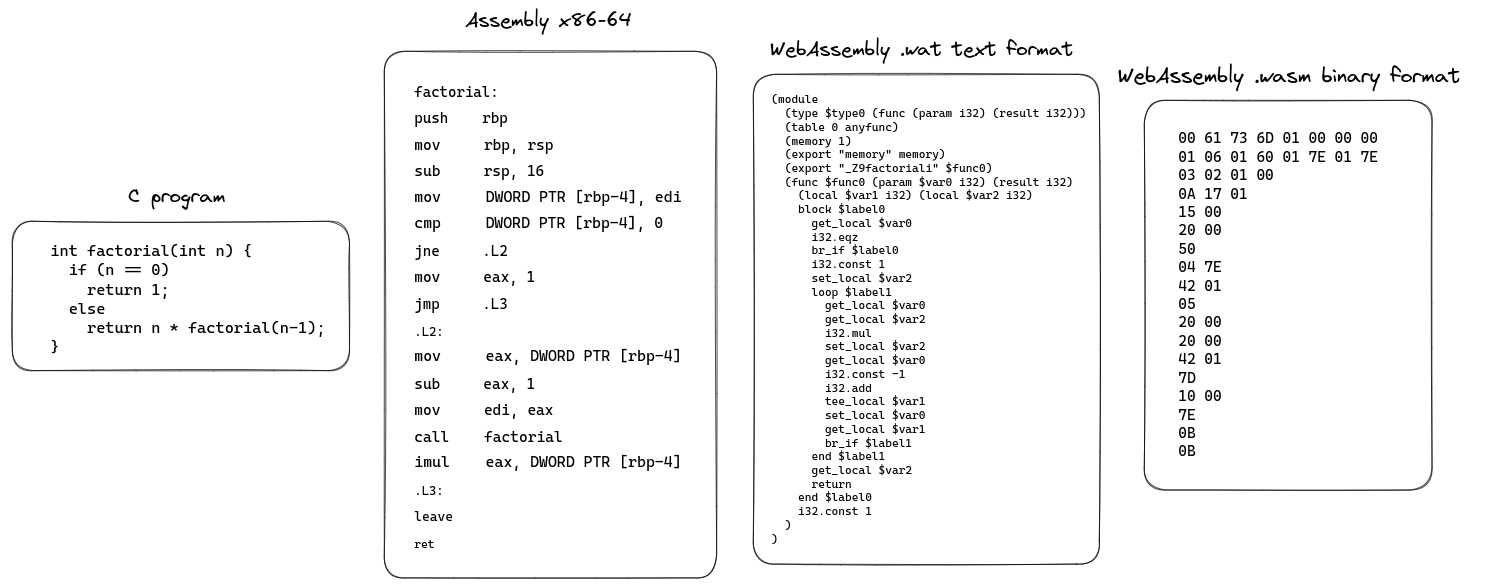
\includegraphics[width=15cm]{./images/3.source_code_wat_wasm.png}
    \label{source_code_wat_wasm}
    \caption{Esempio di una funzione compilata nel modo 'tradizionale', in .wasm e la sua rappresentazione in .wat}
\end{figure}


Come noto, i linguaggi Assembly tradizionali sono strettamente legati all'architettura della CPU sottostante. Ciò significa che ogni programma scritto in Assembly è vincolato alla specifica architettura su cui deve essere eseguito. Pertanto, per rendere un'applicazione compatibile ed eseguibile su diverse macchine, è necessario compilarla per le diverse architetture che si vogliono supportare.
Nel corso degli anni, gli sviluppatori hanno cercato di risolvere questo problema attraverso diverse soluzioni. Ad esempio, il linguaggio Java ha introdotto il motto "Write once, run anywhere". Wasm può essere considerato come una soluzione simile, ma con un vantaggio fondamentale: mentre Java richiede agli sviluppatori di scrivere codice nel linguaggio Java o in linguaggi compatibili con la Java Virtual Machine, per poterlo eseguire su qualsiasi piattaforma, Wasm consente di utilizzare qualsiasi linguaggio di programmazione compilabile in formato .wasm e il risultante codice prodotto può essere eseguito su tutti i browser compatibili.
\\
Tuttavia, gli sviluppatori non si sono limitati ad utilizzare Wasm solo all'interno dei browser. Anche per lo sviluppo di applicazioni tradizionali, Wasm sta diventando sempre più popolare.
In questo contesto, WASI svolge un ruolo cruciale. Mentre all'interno del browser Wasm non ha bisogno di comunicare con il sistema operativo, poiché il browser funge da intermediario, al di fuori di esso, la situazione è diversa. Qui, l'applicazione deve comunicare con il filesystem, creare connessioni di rete, eseguire codice in parallelo e così via, e farlo in modo sicuro, isolando l'applicazione dal sistema operativo sottostante e garantendo che non possa interferire con altri processi o con la memoria del sistema. WASI affronta queste sfide fornendo un insieme di interfacce standardizzate, una \textbf{system interface}, tra le applicazioni Wasm e l'ambiente di esecuzione sottostante.
\clearpage
\section{Cos'è una System Interface?}
Normalmente, le applicazioni non si interfacciano direttamente con le risorse del sistema, ma attraverso il sistema operativo, il cui nucleo è il kernel, che media l'accesso alle risorse. Ciò è necessario per evitare accessi indiscriminati, che potrebbero causare instabilità e problemi di sicurezza. Per questo motivo, il sistema operativo organizza la protezione in strati a livelli crescenti di privilegi. Ogni programma viene eseguito in "user mode" e se vuole eseguire operazioni privilegiate, deve chiedere al kernel di farlo attraverso le system call, che eseguono i controlli necessari prima di permettere l'operazione.
Per semplificare l'accesso alle risorse del sistema, molti linguaggi di programmazione forniscono una libreria standard che definisce un'interfaccia comune, chiamata system interface, indipendente dal sistema operativo sottostante. Ciò significa che gli sviluppatori non devono preoccuparsi dell'implementazione specifica del sistema operativo, poiché possono utilizzare l'interfaccia fornita dal linguaggio di programmazione. Sarà il compilatore a scegliere l'implementazione corretta dell'interfaccia in base al sistema operativo in cui viene eseguita l'applicazione.
\begin{figure}[h]
    \centering
    \captionsetup{justification=centering}
    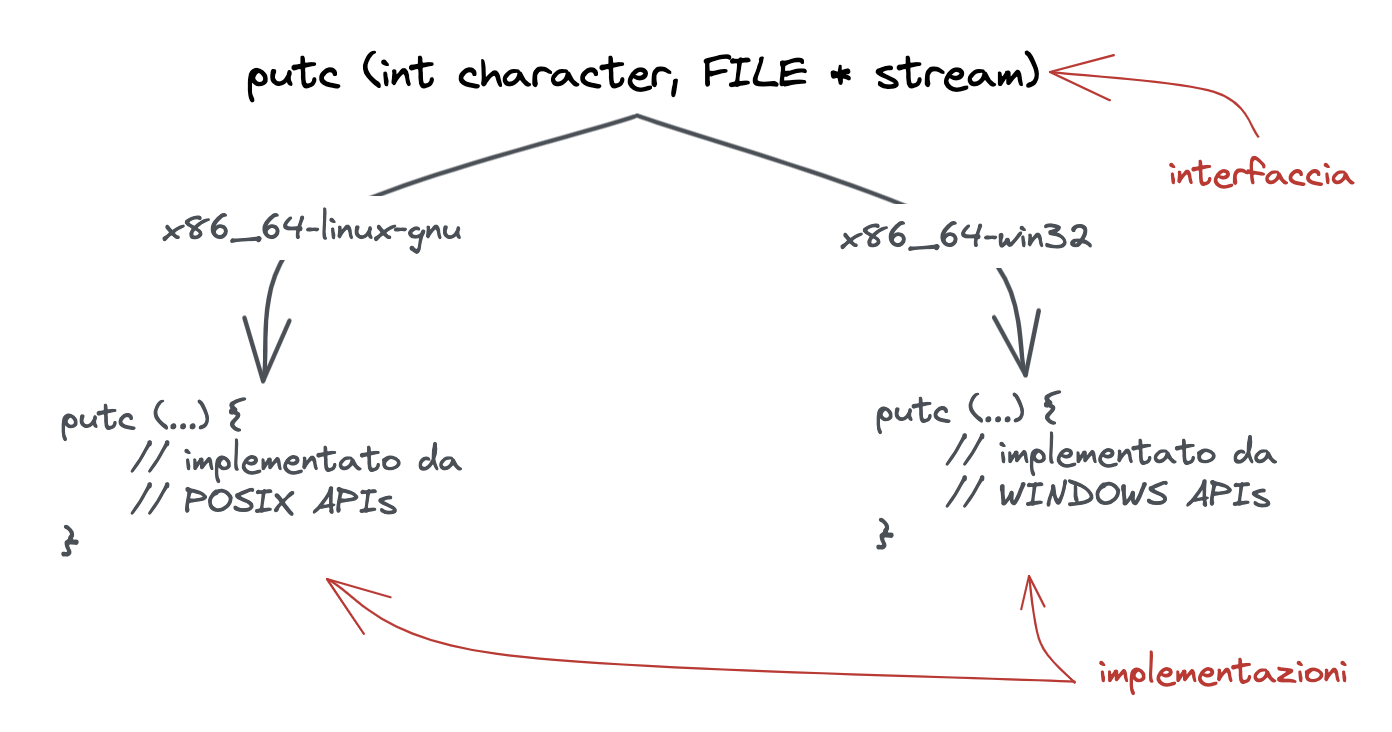
\includegraphics[width=15cm]{./images/5.system-interface-api-to-impl.png}
    \label{system-interface-api-to-impl}
    \caption{System Interface: Dall'API alla sua implementazione}
\end{figure}

Con WebAssembly, invece, è necessario definire un'interfaccia per un sistema operativo concettuale e un runtime che la implementi, poiché non si conosce a priori il sistema operativo su cui verrà eseguito il modulo .wasm.
\begin{figure}[H]
    \centering
    \captionsetup{justification=centering}
    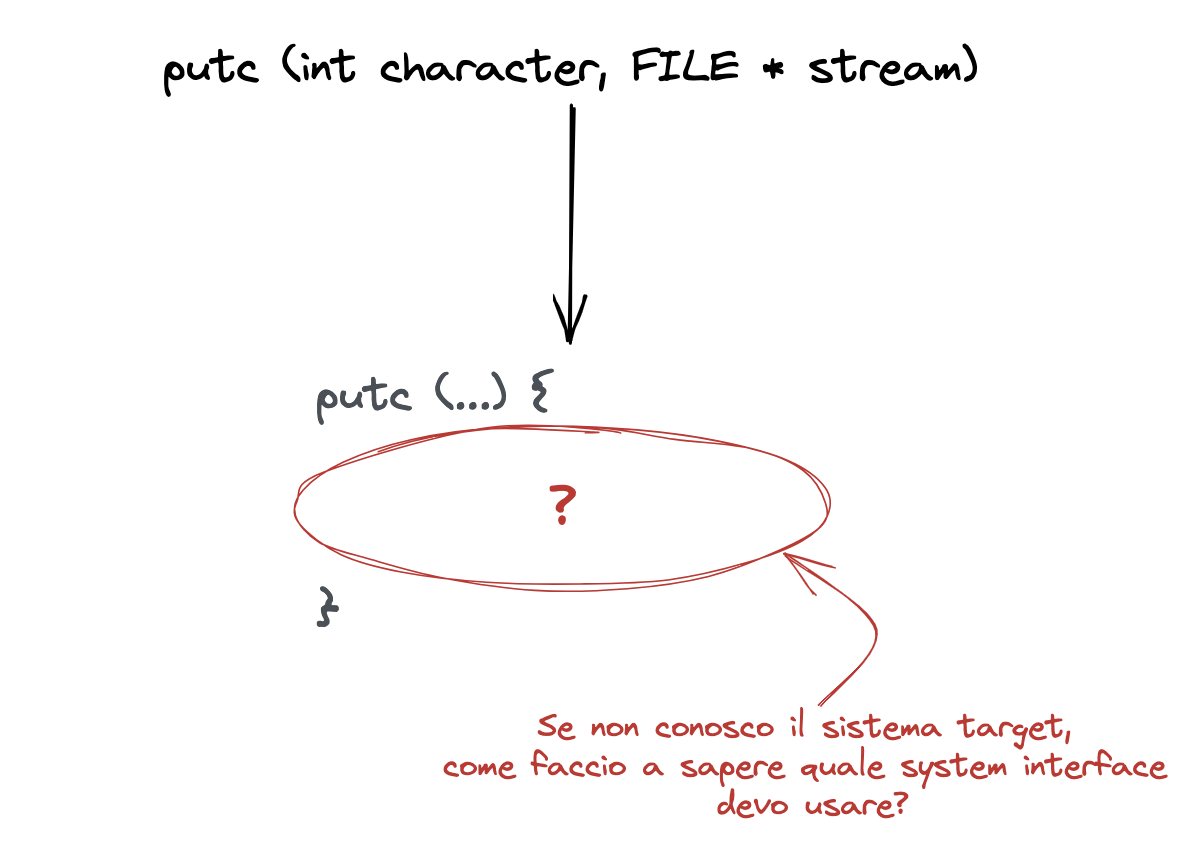
\includegraphics[width=15cm]{./images/5a.wasi_sys_interface.png}
    \label{system-interface-conceptual-sys}
    \caption{Una System Interface per un sistema operativo concettuale}
\end{figure}
Questa interfaccia deve essere poi implementata dai runtime capaci di eseguire effettivamente i moduli wasm.


\section{Stato dell'arte}
Esistono già vari runtime che permettono di eseguire codice WebAssembly (wasm) al di fuori del browser, molti dei quali seguono le interfacce definite dallo standard WASI in modo più o meno stretto. Ci sono runtime specializzati in diverse categorie, ma anche quelli che mirano ad essere più specifici e a coprire tutto lo standard nella sua completezza.
\\
Ogni nuova interfaccia inserita nello standard, detta WASI API, segue un rigoroso percorso diviso in 6 fasi\footnote{\url{https://github.com/WebAssembly/meetings/blob/main/process/phases.md}} prima di essere standardizzata:
\begin{itemize}
    \item \textbf{Pre-Proposal}: presentazione dell'idea iniziale e valutazione della sua fattibilità e rilevanza dalla comunità degli sviluppatori.
    \item \textbf{Feature Proposal}: presentazione dettagliata di una nuova funzionalità o modifica all'API esistente, valutata dalla comunità degli sviluppatori.
    \item \textbf{Spec Text Available}: scrittura del testo di specifica proposto con la descrizione dettagliata di come la nuova funzionalità o modifica dell'API dovrebbe essere implementata.
    \item \textbf{Implementation Phase}: fase di implementazione, in cui gli sviluppatori creano un'implementazione funzionante della funzionalità o modifica dell'API.
    \item \textbf{Standardize}: la nuova funzionalità o modifica dell'API viene sottoposta a una revisione formale per verificare che l'implementazione soddisfi i requisiti specificati nella proposta e nel testo della specifica proposto.
    \item \textbf{The Feature is Standardized}: la funzionalità o modifica dell'API viene aggiunta alla specifica ufficiale e diventa disponibile per gli sviluppatori.
\end{itemize}


Attualmente, nessuna delle nuove interfacce inserite nello standard WASI API ha superato la fase 2\footnote{\url{https://github.com/WebAssembly/WASI/blob/main/Proposals.md}}.
In ogni caso, è importante notare che ogni runtime sviluppa la propria implementazione delle funzionalità necessarie per il suo specifico scopo, anche se non segue strettamente lo standard WASI. Ad esempio, l'API per le socket è ancora in fase 1 (Feature Proposal), ma è già disponibile in alcuni runtime che ne hanno bisogno. Un esempio di runtime che segue questa filosofia è WasmEdge\footnote{\url{https://github.com/WasmEdge/WasmEdge}}, che adotta lo standard WASI per le API già pronte per essere implementate ma prende decisioni diverse per quanto riguarda i moduli ancora in fase di discussione.

\section{WasmEdge}
In questo documento ci concentreremo sull'utilizzo di WasmEdge come runtime per l'esecuzione di codice WebAssembly sul cloud. WasmEdge è un runtime sviluppato con l'obiettivo di portare la tecnologia wasm nell'ambito del cloud computing, e quindi di rendere possibile l'esecuzione di applicazioni wasm in ambienti distribuiti e scalabili.
\\
Inoltre, WasmEdge è l'unico runtime (ad oggi) in grado di essere utilizzato in combinazione con Docker, uno dei più diffusi strumenti di containerizzazione. Docker ha recentemente lanciato il supporto ai container wasm\cite{docker-wasm-tech-preview}, il che significa che ora è possibile utilizzare i container Docker per eseguire applicazioni wasm. Questo è un importante passo avanti nel mondo del cloud computing, perchè, come vedremo, i container wasm risultano essere più leggeri e veloci in determinati contesti.
\\
Per comprendere meglio l'impatto che WASI potrebbe avere nel mondo del cloud computing:
\begin{quote}
    If WASM+WASI existed in 2008, we wouldn't have needed to create Docker. That's how important it is. Webassembly on the server is the future of computing. A standardized system interface was the missing link. Let's hope WASI is up to the task!
    \\
    \textit{Solomon Hykes - Former Docker Founder}\footnote{\url{https://twitter.com/solomonstre/status/1111004913222324225}}
\end{quote}

Significa che Wasm rimpiazzerà completamente docker? No, ma è un'ulteriore tecnologia che si aggiunge a quelle già esistenti, con i propri punti di forza e di debolezza.
\begin{quote}
    “So will wasm replace Docker?” No, but imagine a future where Docker runs linux containers, windows containers and wasm containers side by side. Over time wasm might become the most popular container type. Docker will love them all equally, and run it all :)
    \\
    \textit{Solomon Hykes - Former Docker Founder}\footnote{\url{https://twitter.com/solomonstre/status/1111113329647325185}}
\end{quote}

Nel documento utilizzeremo quindi WasmEdge in combinazione con Docker, analizzando i vantaggi e le limitazioni di questa soluzione.